% Document template suitable for use as a latex master-file for masters
% thesis in University of Turku Department of Future Technologies. 

% This template is synced with the gitlab template.
% Works with sharelatex / pdflatex / xelatex

% --

% HOW TO USE?
%
% Want to write a thesis? Clone this template
% Kirjoitatko tutkielmaa? Kloonaa tämä pohja

% Want to fix something in the template? Send a
% merge request @ https://gitlab.utu.fi/jmjmak/thesis
% Haluatko korjata jotain alkup. pohjassa? Lähetä
% korjauspyyntö @ https://gitlab.utu.fi/jmjmak/thesis

% --

% Relies on utuftthesis.cls for the document class definitions.

% Traditionally the best places to learn (La)TeX are probably the manual
% pages for each package
%   http://www.ctan.org/ 
% and
%  http://www.ctan.org/tex-archive/info/lshort/english/lshort.pdf

% This new version (2.0) should be compatible with xelatex and biblatex
% which means that all source files can freely use normal UTF-8 text
% without resorting to ""legacy hacks".
%
%
% The utuftthesis.cls defines a new thesis class, which is based on
% the report class. It supports these new named parameters:
% paper: a4paper
% version: draft / final (draft shows [draft] in the header)
% language: provide a language (finnish,english) as a parameter to
%          change the general document appearance and hyphenation
% hidechapters: show (false) or hide (true) the chapter/luku text at the
%               beginning of each Chapter
% includereferences: include reference pages when calculating the total
%                    number of pages
\documentclass[paper=a4paper,version=final,language=finnish,hidechapters=false,includereferences=false]{utuftthesis}

%\usepackage{hyperref}

\bibliography{Bibliografia}
                 
\begin{document}

% your name
\author{My Name}

% the name of the thesis (used automatically on several pages)
\title{Name of Thesis}

% publication year
\pubyear{2018}

% publication month 1-12
\pubmonth{6}

% laboratory name
\publab{Labran Nimi}{Laboratory Name}

% supports magic values: tkk, luk, gradu & di
\pubtype{tkk}

% not necessary. supports 1..n supervisors :)
%\supervisors{First Supervisor, Second Supervisor}

% Generate the title page 
\maketitle

% Include the abstract (+ second abstract if any)

\keywords{tähän, lista, avainsanoista}
% TODO: good/bad keywords

\keywordsen{here, a, list, of, keywords}
\begin{abstract}
Tarkempia ohjeita tiivistelmäsivun laadintaan läytyy opiskelijan yleisoppaasta,
josta alla lyhyt katkelma.

Bibliografisten tietojen jälkeen kirjoitetaan varsinainen tiivistelmä.
Sen on oletettava, että lukijalla on yleiset tiedot aiheesta. Tiivistelmän
tulee olla ymmärrettävissä ilman tarvetta perehtyä koko tutkielmaan.
Se on kirjoitettava täydellisinä virkkeinä, väliotsakeluettelona.
On käytettävä vakiintuneita termejä. Viittauksia ja lainauksia tiivistelmään
ei saa sisällyttää, eikä myäskään tietoja tai väitteitä, jotka eivät
sisälly itse tutkimukseen. Tiivistelmän on oltava mahdollisimman ytimekäs
n. 120–250 sanan pituinen itsenäinen kokonaisuus, joka mahtuu ykkäsvälillä
kirjoitettuna vaivatta yhdelle tiivistelmäsivulle. Tiivistelmässä tulisi ilmetä
mm.  tutkielman aihe tutkimuksen kohde, populaatio, alue ja tarkoitus
käytetyt tutkimusmenetelmät (mikäli tutkimus on luonteeltaan teoreettinen
ja tiettyyn kirjalliseen materiaaliin, on mainittava tärkeimmät lähdeteokset;
mikäli on luonteeltaan empiirinen, on mainittava käytetyt metodit)
keskeiset tutkimustulokset tulosten perusteella tehdyt päätelmät ja
toimenpidesuositukset.
\end{abstract}

\begin{abstracten}
Second abstract in english (in case the document main language is
not english)
\end{abstracten}



% empty pagestyle for table of contents etc. 
%
% the redefinition of plain style works also for 1st pages of chapters,
% which is the default in report class. Just state \thispagestyle{empty}
% after \chapter{something} if you want empty style for the 1st pages. 
%
\pagestyle{empty}
\fancypagestyle{plain}{
  \fancyhf{}
  \renewcommand{\headrulewidth}{0 pt}
}

% roman numbering for table of contents etc.
\pagenumbering{roman}

% insert table of contents, list of figures, list of tables
%
% setting the counter to zero effectively removes the page number from
% the toc, lof etc. entries in the toc since there is no roman numeral
% for zero ;-) (if you want them without numbering)
%
%\setcounter{page}{0}
\tableofcontents
\clearpage
%\setcounter{page}{0}
%\listoffigures 
%\clearpage
%\setcounter{page}{0}
%\listoftables

% possibly insert 'list of acronyms'
%
%   - create a chapter called List Of Acronyms (or whatever), which
%     should contain all your acronym definitions, e.g. 
%     \chapter{List Of Acronyms} 
%   - the secnumdepth trickery is needed because acronyms are as a
%     standard chapter and we are faking '\listofacronyms'
%
%\setcounter{secnumdepth}{-1}
%\input{your acronym chapter's file name}
%\setcounter{secnumdepth}{2}

% setup page numbering, page counter, etc.
\startpages

%%%%%%%%%%%%%%%%%%%%%%%%%%%%%%%%%%%%%%%%%%%%%%%%%%%%%%%%%%%%%%%%%%%%%%%%%%%
%
% Thesis starts here. Create a new tex file for each chapter and input it
% below. You may encounter errors if you use å, ä, ö or <space> characters
% in referred names.
%
% Good luck!
%
%%%%%%%%%%%%%%%%%%%%%%%%%%%%%%%%%%%%%%%%%%%%%%%%%%%%%%%%%%%%%%%%%%%%%%%%%%%

\chapter{Johdanto} \label{Johdanto}

Viittaaminen lukuun \ref{Johdanto}, toiseen lukuun \ref{Toinen luku},
alilukuun \ref{Alaotsikko}, tätä alempaan lukuun \ref{Alempiotsikko},
alimpaan lukuun \ref{Alinotsikko}, kuvaan \ref{Kuva esimerkki} ja
tauluun \ref{Tauluesimerkki}.

Kuva liitetään seuraavasti. ShareLaTeXin autocomplete rakentaa koko
begin-end blockin yleensä puolestasi.

\begin{figure}
\centering 
\includegraphics[width=0.5\textwidth]{kuvat/utulogoen}
\caption{Kuvan otsikko}
\label{Kuva esimerkki} 
\end{figure}

Taulukkoja tehdään seuraavasti.

\begin{table}
\begin{centering}
\caption{Taulukon otsikko tulee taulun yläpuolelle}
\begin{tabular}{l|c|r|}
Taulun  & elementit  & erotetaan \tabularnewline
\hline 
toisistaan  & et-merkillä  & \tabularnewline
soluja voi myös  &  & jättää tyhjäksi \tabularnewline
\end{tabular}
\par\end{centering}
\centering{}\label{Tauluesimerkki}
\end{table}

Kirjallisuusviitteet lisätään bib-muodossa bibliografia tiedostoon
ja niihin viitataan niiden ID:llä, joka on bib-muodon ensimmäinen
kenttä \cite{crawley2007write}.

\section{Alaotsikko}

\label{Alaotsikko}

Uskonpuhdistuksen myötä suomi tuli koko jumalanpalveluksen kieleksi.
Raamattu ja liturgiset kirjat oli siksi saatava suomeksi. Maahan tarvittiin
suomea osaavia pappeja; kouluihin piti sen vuoksi saada suomen kielen
opetusta, ja sitä varten tarvittiin oppikirjoja. Nämä asiat olivat
nuoren Mikael Agricolan kannustimena, kun hän aloitti elämäntyönsä
suomen kirjakielen kehittäjänä.

Agricola opiskeli monen muun suomalaisnuorukaisen tavoin Wittenbergissä.
Jo ennen Wittenbergin vuosia hän oli saanut valmiiksi Abckirian ja
Rucouskirian. Abckiria oli tarkoitettu oppikirjaksi. Se sisälsi aakkoset,
tavausharjoituksia ja katekismuksen. Laajassa Rucouskiriassa on rukousten
lisäksi Raamatun tekstejä, muun muassa 41 psalmia. Alussa on monipuolinen
kalendaario, joka sisältää esimerkiksi ruokailu- ja terveydenhoito-ohjeita
ja jopa jonkinlaisen horoskoopin.

Uutta testamenttia Agricola käänsi Wittenbergissä apuneuvoinaan kaksi
latinalaista, kaksi saksalaista ja kaksi ruotsalaista käännöstä. Se
Wsi Testamenti ilmestyi 1548. Kirjan sanasto ja muoto-oppi on siinä
määrin epäyhtenäistä, että on arveltu, että käännöksellä on Agricolan
lisäksi ollut myös muita viimeistelijöitä.

Agricolan osuus 1551 ilmestyneen Psalttarin psalmisuomennoksista on
epäselvä. Suuri osa psalmeista onkin todennäköisesti suomennettu Turun
koulussa Paavali Juustenin johdolla. Juusten itse on kirjoittanut
Psalttarista Suomen piispainkronikassa (suom. Simo Heininen): ``Mutta
ei ole ollenkaan väliä, kenen nimissä se on julkaistu, sillä se on
käännetty, jotta siitä olisi suurta hyötyä Suomen kansalle.'' Pääosa
Psalttarin esipuheista on Agricolan omaa tekstiä. Runomuotoiseen esipuheeseen
sisältyy ansiokas luettelo suomalaisten pakanallisista jumalista.
Agricola suomensi myös osia Mooseksen kirjoista ja profeetoista. Hänen
nimissään on ilmestynyt suomeksi noin 2/5 Raamatusta. Toinen esimerkki
viittaamisesta, jossa myös cite komennon tagi löytyy Bibliografia.bib
tiedostosta \cite{puasuareanu2009survey}.

\subsection{Alempiotsikko}

\label{Alempiotsikko}

Lorem ipsum dolor sit amet, consectetur adipiscing elit. Etiam eget
tellus porttitor, tempus lacus non, pellentesque ligula. Donec sit
amet erat condimentum, feugiat mi accumsan, euismod quam.

Mauris laoreet maximus aliquet. Mauris at gravida elit. Ut nec lobortis
elit. Sed lacinia nisi in ex sollicitudin, ac consequat lacus imperdiet.
Etiam et velit eu lacus maximus faucibus.

\subsubsection{Alinotsikko, joka ei näy sisällysluettelossa}

\label{Alinotsikko}

Lorem ipsum dolor sit amet, consectetur adipiscing elit. Etiam eget
tellus porttitor, tempus lacus non, pellentesque ligula. Donec sit
amet erat condimentum, feugiat mi accumsan, euismod quam.

\paragraph{Otsikko tekstissä, joka ei näy sisällysluettelossa}

Mauris laoreet maximus aliquet. Mauris at gravida elit. Ut nec lobortis
elit. Sed lacinia nisi in ex sollicitudin, ac consequat lacus imperdiet.
Etiam et velit eu lacus maximus faucibus. Vestibulum ante ipsum primis
in faucibus orci luctus et ultrices posuere cubilia Curae; Donec vulputate
tellus ullamcorper odio sodales, non scelerisque neque eleifend. 

\chapter{Toisen luvun otsikko} \label{Toinen luku}

Tässä luvussa tarkastellaan kahden kuvan upottamista samaan kelluvaan
kuvaympäristöön (Kuva \ref{fig:Optimointia-kahdella-eri}).

\begin{figure}[tbh]
\subfloat[Käynnistysajan optimointi Nailgunilla.]{\begin{centering}
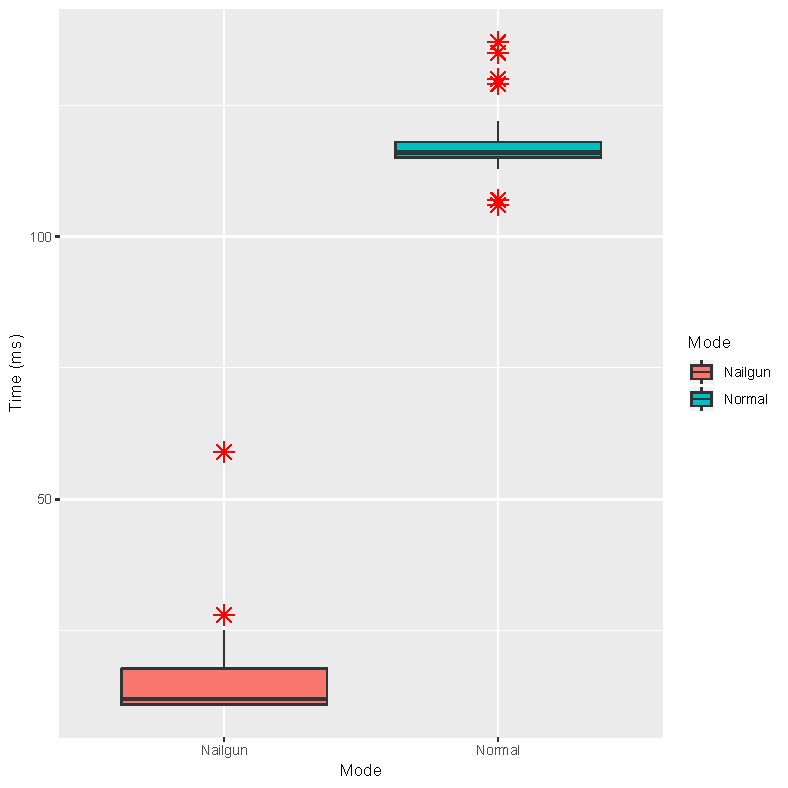
\includegraphics[width=0.45\textwidth]{kuvat/nailgun.pdf}
\par\end{centering}
}\subfloat[Koon optimointi Proguardilla.]{\begin{centering}
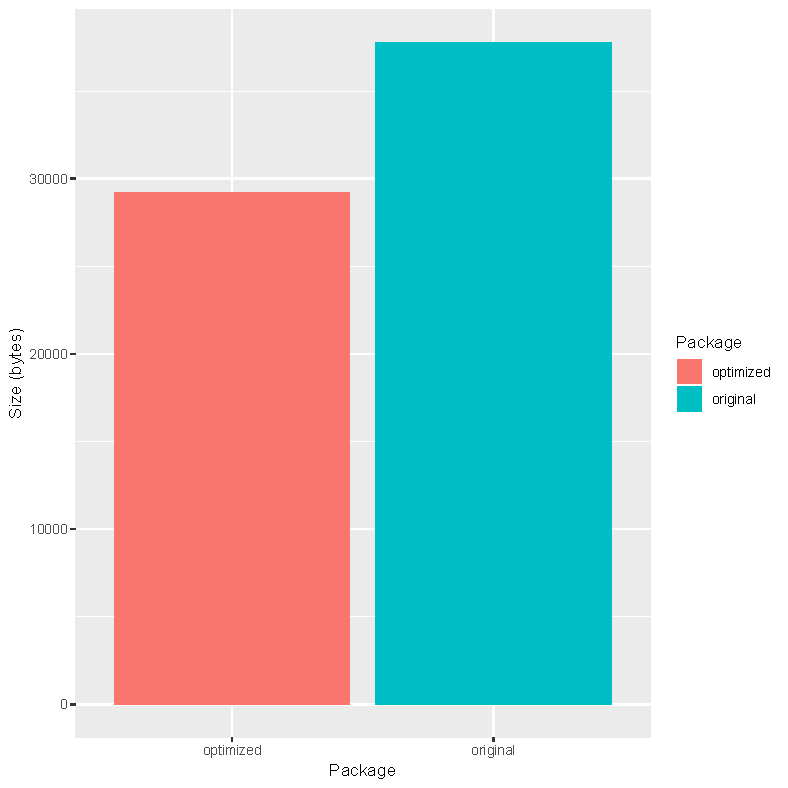
\includegraphics[width=0.45\textwidth]{kuvat/proguard.pdf}
\par\end{centering}
}\caption{Optimointia kahdella eri tavalla.\label{fig:Optimointia-kahdella-eri}}

\end{figure}


%\input{file_name_of_chapter_x}
%\input{file_name_of_chapter_y}

% insert references
\printbibliography
%%%%%%%%%%%%%%%%%%%%%%%%%%%%%%%%%%%%%%%%%%%%%%%%%%%%%%%%%%%%%%%%%%%%%%%%%%%
%
% Almost there....
%
%%%%%%%%%%%%%%%%%%%%%%%%%%%%%%%%%%%%%%%%%%%%%%%%%%%%%%%%%%%%%%%%%%%%%%%%%%%

% make sure pagecount is correct even if references overflow to a new page
\pagebreak\addtocounter{page}{-1}

% don't include this if appendices are not present
%\appendices

\appchapter{Liitedokumentti}
Tässä esimerkki\newpage kaksisivuisesta liitteestä.

\appchapter{Liitedokumentti 2}
Tässä esimerkki\newpage toisesta kaksisivuisesta liitteestä.

%\appchapter{Liitedokumentti 3}
%Tässä esimerkki yksisivuisesta liitteestä.

% create your appendix chapters with command \appchapter{some name} instead
% of \chapter{some name} for the automagic page counting to work
%\input{file name of appchapter xxx}
%\input{file name of appchapter yyy}
%\input{file name of appchapter zzz}
%\input{and so on}

%%%%%%%%%%%%%%%%%%%%%%%%%%%%%%%%%%%%%%%%%%%%%%%%%%%%%%%%%%%%%%%%%%%%%%%%%%%
%
% main document ends here
%
%%%%%%%%%%%%%%%%%%%%%%%%%%%%%%%%%%%%%%%%%%%%%%%%%%%%%%%%%%%%%%%%%%%%%%%%%%%

\end{document}
